\documentclass{article} % For LaTeX2e
\usepackage{iclr2024_conference,times}

\usepackage[utf8]{inputenc} % allow utf-8 input
\usepackage[T1]{fontenc}    % use 8-bit T1 fonts
\usepackage{hyperref}       % hyperlinks
\usepackage{url}            % simple URL typesetting
\usepackage{booktabs}       % professional-quality tables
\usepackage{amsfonts}       % blackboard math symbols
\usepackage{nicefrac}       % compact symbols for 1/2, etc.
\usepackage{microtype}      % microtypography
\usepackage{titletoc}

\usepackage{subcaption}
\usepackage{graphicx}
\usepackage{amsmath}
\usepackage{multirow}
\usepackage{color}
\usepackage{colortbl}
\usepackage{cleveref}
\usepackage{algorithm}
\usepackage{algorithmicx}
\usepackage{algpseudocode}

\DeclareMathOperator*{\argmin}{arg\,min}
\DeclareMathOperator*{\argmax}{arg\,max}

\graphicspath{{../}} % To reference your generated figures, see below.

\title{Adaptive Stochastic Depth: Dynamic Regularization via Online Loss Monitoring}

\author{LLM\\
Department of Computer Science\\
University of LLMs\\
}

\newcommand{\fix}{\marginpar{FIX}}
\newcommand{\new}{\marginpar{NEW}}

\begin{document}

\maketitle

\begin{abstract}
% This paragraph motivates dynamic regularization for Transformers, explains the challenge of fixed schedules,
% presents our online EMA‑based controller, and summarises the empirical results showing improved speed without harming loss.
Adaptive regularization is crucial for training deep Transformer models without overfitting, yet classical dropout and fixed stochastic depth schedules offer limited control over the trade-off between capacity and speed. In this work, we introduce \textit{Adaptive Stochastic Depth}, a lightweight online controller that dynamically adjusts the probability of skipping Transformer blocks during training. At each evaluation interval, we compute an exponential moving average of the validation loss and compare its relative improvement with a threshold \(\varepsilon\). If the improvement is insufficient, the block‑skip probability \(p\) is increased by a fixed step \(\delta\) (capped at \(p_{\text{max}}\)), encouraging stronger regularization; otherwise \(p\) is decreased, allowing the model to retain more capacity. Our method requires no additional learned parameters, introduces negligible overhead, and can be retrofitted to existing architectures with a single non‑persistent buffer. Experiments on three character‑level language modeling benchmarks (shakespeare\_char, enwik8, and text8) demonstrate that Adaptive Stochastic Depth consistently matches the validation loss of a fixed‑probability baseline while drastically reducing training time. On the larger enwik8 and text8 datasets, training time is reduced by more than $15\times$ and the probability trajectory evolves smoothly with the loss landscape, confirming that the controller effectively reacts to overfitting signals. These results suggest that simple, loss‑driven adaptation can serve as a practical drop‑in replacement for hand‑crafted stochastic depth schedules, providing both robustness and efficiency in large‑scale language model training.
\end{abstract}

\section{Introduction}
\label{sec:intro}

% This paragraph sets the broad context: Transformer language models and the need for regularization.
Deep Transformer architectures \citep{vaswani2017attention} have become the backbone of modern language modeling, achieving state-of-the-art performance across a wide range of natural language tasks \citep{radford2019language,karpathy2023nanogpt}.
However, when training such models on moderate-sized datasets, overfitting becomes a significant concern, motivating the use of various regularization techniques.  
Dropout and layer normalization \citep{ba2016layer} are among the most popular, but stochastic depth—stochastically dropping entire blocks during training—has recently gained traction as an effective regularizer that enforces distributed representations and reduces co-adaptation between layers.
Despite its benefits, stochastic depth is typically applied with a fixed drop probability or a linearly increasing schedule, both of which are static hyperparameters that cannot adapt to the evolving loss landscape during training.

% This paragraph explains why the problem is hard: the optimal drop rate changes as training progresses and differs per dataset.
Choosing an appropriate drop schedule is challenging because the optimal trade‑off between model capacity and regularization varies throughout training.
A drop rate that is too small early in training may fail to prevent overfitting, while a rate that is too large later can needlessly reduce representational capacity and degrade final performance.
Furthermore, different datasets and architectures require distinct schedules, making ad‑hoc manual tuning both time‑consuming and brittle.
Ideally, the regularization strength would automatically adjust in response to real‑time signals that indicate whether the model is overfitting or underfitting.

% This paragraph introduces our contribution: an online EMA‑based controller that adjusts the stochastic depth probability according to the validation loss trend.
We address this challenge with \textit{Adaptive Stochastic Depth}, a lightweight controller that monitors the validation loss during training and modulates the block‑skip probability online.
At the end of each evaluation interval, we compute an exponential moving average (EMA) of the validation loss and evaluate its relative improvement.
If the improvement falls below a threshold, the controller interprets the stagnation as a sign of overfitting and increases the drop probability \(p\); otherwise it decreases \(p\), allowing the model to retain more capacity.
Crucially, the method requires no additional learned parameters, introduces negligible computational overhead, and can be retrofitted to any existing Transformer architecture through a single non‑persistent buffer.

% This paragraph lists the paper's contributions as bullet points.
Our main contributions are:

\begin{itemize}
    \item We propose \textbf{Adaptive Stochastic Depth}, a simple online control algorithm that dynamically adjusts the stochastic depth probability based on the trajectory of the validation loss.
    \item We provide an efficient implementation using only a non‑persistent buffer, requiring only three simple hyperparameters: the improvement threshold \(\varepsilon\), the probability step \(\delta\), and the maximum probability \(p_{\text{max}}\).
    \item We conduct experiments on three character‑level language modeling benchmarks (shakespeare\_char, enwik8, and text8) using the nanoGPT architecture \citep{karpathy2023nanogpt}. The adaptive controller reduces training time by 17\% on shakespeare\_char and by more than \(15\times\) on enwik8 and text8, while the validation loss remains within \(0.4\) nats of the no‑drop baseline on the larger datasets.
    \item We show that the drop probability evolves smoothly and reacts to overfitting signals, yielding trajectories that are interpretable and consistent across runs.
\end{itemize}

% This paragraph outlines the experimental setup and previews the quantitative results that will be presented later.
To validate our approach, we train small GPT‑style models on the three datasets and compare the proposed adaptive schedule against a standard baseline trained without stochastic depth.
As detailed in Section~\ref{sec:results}, Adaptive Stochastic Depth matches the validation loss of the baseline on shakespeare\_char (1.47 vs.\ 1.47) and incurs a validation loss increase of less than \(0.4\) nats on the larger datasets, while achieving training‑time accelerations of up to \(15.9\times\) on enwik8 and up to \(15.0\times\) on text8.
Inference throughput on the same models improved by 43\% on shakespeare\_char and 73\% on enwik8, but decreased by 28\% on text8.
These results demonstrate that simple, loss‑driven adaptation can serve as a practical drop‑in replacement for hand‑crafted stochastic depth schedules, offering both robustness and efficiency with minimal tuning.

\section{Related Work}
\label{sec:related}

% This section compares our approach with existing regularization techniques and adaptive schedules.
% Paragraph 1: standard static regularizers for Transformers.
Regularization is essential in training deep Transformer models \citep{vaswani2017attention}. The most common techniques include dropout \citep{goodfellow2016deep}, weight decay \citep{loshchilov2017adamw}, and layer normalization \citep{ba2016layer}. While these methods are effective, they rely on fixed hyperparameters tuned before training; they cannot adapt to the evolving risk of overfitting over the course of training.

% Paragraph 2: stochastic depth and its static schedules.
Stochastic depth, where entire network blocks are skipped during training, was originally proposed for convolutional architectures and has recently been adopted in Transformer language models \citep{karpathy2023nanogpt}. The standard practice is to use a constant drop probability or a linearly increasing schedule. Although these strategies can improve generalization, they require the practitioner to manually search for a probability trajectory that is appropriate for a given architecture and dataset. A poorly chosen schedule can negate the benefits of stochastic depth or even harm final performance.

% Paragraph 3: adaptive dropout methods and comparison to our controller.
A few attempts have been made to learn the dropout probability adaptively, for example by treating it as a variational parameter or by using concrete distributions that can be optimized with gradient descent. These approaches introduce additional learnable parameters and modify the training objective, increasing both the conceptual complexity and the computational cost. In contrast, our Adaptive Stochastic Depth controller operates outside the optimization loop. It uses only an exponential moving average of the validation loss—a signal that is cheap to compute and already available in most training pipelines—to decide when to strengthen or weaken regularization. It requires no gradient with respect to the regularization hyperparameter, stores no new parameters in the model’s optimizer state, and can be implemented with a single non‑persistent buffer.

% Paragraph 4: relation to adaptive learning‑rate schedules.
Finally, we note that adaptive learning‑rate schedules, such as Adam \citep{kingma2014adam} and AdamW \citep{loshchilov2017adamw}, adjust the step size based on gradient history but do not modify the model’s effective capacity. Our controller therefore complements these optimizers by adding a capacity‑aware adaptive mechanism that is orthogonal to the learning rate schedule.

% Overall, the related work demonstrates that loss‑based online adaptation of the stochastic depth probability is an underexplored direction, and our method fills this gap with a practical, lightweight solution.

\section{Background}
\label{sec:background}

% This paragraph reviews the Transformer architecture and its autoregressive language modeling objective.
The Transformer architecture \citep{vaswani2017attention} has emerged as the dominant paradigm for sequence modeling tasks. 
A Transformer consists of an embedding layer that maps input tokens to dense vectors, a sinusoidal positional encoding that injects order information, and a stack of \(L\) identical blocks. Each block applies multi-head self-attention followed by a position-wise feedforward network, both surrounded by residual connections and layer normalization \citep{ba2016layer}. 
For autoregressive language modeling, the model is trained to predict the next token given a context window, minimizing the standard cross-entropy loss over the training distribution.

% This paragraph describes stochastic depth as a regularization technique and its typical schedules.
To combat overfitting, deep models rely on a variety of regularizers, including dropout \citep{goodfellow2016deep}, weight decay \citep{loshchilov2017adamw}, and stochastic depth. 
Stochastic depth (also known as block dropout) randomly drops entire Transformer blocks during each training forward pass, while at inference time all blocks remain active. 
Formally, we assign a single probability \(p\) shared across all layers. For block \(i\) with input \(x^{(i)}\), the block is skipped with probability \(p\):
\[
\tilde{x}^{(i)} = \begin{cases}
x^{(i)} + \mathrm{block}_i\bigl(\mathrm{LN}(x^{(i)})\bigr), & \text{with probability } 1-p,\\[4pt]
x^{(i)}, & \text{with probability } p.
\end{cases}
\]
Here \(\mathrm{LN}\) denotes layer normalization and \(\mathrm{block}_i\) encapsulates the self-attention and feedforward sublayers. 
Traditionally, \(p\) is either kept constant during training or increased linearly from zero to a predefined maximum. 
The optimal schedule depends heavily on the dataset, the model size, and the training phase, making manual tuning both tedious and brittle.

% This subsection formalizes the training problem and introduces the notation for our method.
\subsection{Problem Setting}
\label{sec:problem}

We consider a Transformer language model parameterized by \(\theta\) and trained on a dataset \(\mathcal{D}\) using the AdamW optimizer \citep{loshchilov2017adamw} with a cosine learning rate schedule. 
Let \(\ell(\theta;x,y)\) denote the per-token cross-entropy loss for a mini-batch \((x,y)\). 
At each optimization step \(t\) (measured in iterations), the model encounters a new mini-batch and updates \(\theta\) via a standard gradient-based step. 
In addition to the usual training loop, we maintain a stochastic‑depth probability \(p_t\in[0,1]\) that governs the chance of skipping individual Transformer blocks during the forward pass.

After every \(K\) training iterations we evaluate the model on a held‑out validation set, obtaining the validation loss \(\mathcal{L}_{\text{val}}(\theta_t)\). 
We compute an exponential moving average (EMA) of the validation loss,
\[
\overline{\mathcal{L}}_t = \alpha\,\mathcal{L}_{\text{val}}(\theta_t) + (1-\alpha)\,\overline{\mathcal{L}}_{t-K},
\]
where \(\alpha\in(0,1)\) is a fixed smoothing coefficient and \(\overline{\mathcal{L}}_{t-K}\) is the EMA value from the previous evaluation. 
The controller then updates \(p_t\) based on the relative improvement of this smoothed loss. 
The goal is to obtain a sequence \(\{p_t\}\) that automatically balances model capacity and regularization, reducing total wall‑clock training time while keeping the final validation loss close to that of an unregularized model.

We highlight three key design choices: (1) the controller uses only a non‑persistent buffer to store \(p_t\) and the EMA; (2) the decision rule compares the relative improvement against a threshold \(\varepsilon\) and adjusts \(p_t\) by a fixed step size \(\delta\); and (3) we cap the probability at a maximum value \(p_{\text{max}}\). 
These simple choices make the method easy to implement and require no task‑specific tuning beyond the three hyperparameters \(\varepsilon\), \(\delta\), and \(p_{\text{max}}\).

\section{Method}
\label{sec:method}

We propose \textit{Adaptive Stochastic Depth}, a lightweight online controller that dynamically adjusts the block‑skip probability \(p_t\) of a Transformer model (see Section~\ref{sec:problem}) during training. The core idea is to monitor the trajectory of the validation loss and, based on its rate of improvement, decide whether the current regularization strength is sufficient. When the smoothed validation loss stagnates—indicating possible overfitting—the controller raises \(p_t\) to strengthen regularization; when the loss continues to improve, it lowers \(p_t\) to recover model capacity. Because the controller uses only the validation loss, it reacts directly to overfitting signals without being misled by noise in the training loss.

The update rule is applied at the end of each evaluation interval of length \(K\) iterations. Let \(\mathcal{L}_{\text{val}}(\theta_t)\) be the current validation loss. We maintain an exponential moving average (EMA) according to
\[
\overline{\mathcal{L}}_t = \alpha\,\mathcal{L}_{\text{val}}(\theta_t) + (1-\alpha)\,\overline{\mathcal{L}}_{t-K},
\]
where \(\alpha\in(0,1)\) is a smoothing coefficient (we use \(\alpha=0.5\) throughout). Denote \(\overline{\mathcal{L}}_{\text{prev}} = \overline{\mathcal{L}}_{t-K}\) the EMA from the previous evaluation. We then compute the relative improvement of the smoothed loss as
\[
\Delta_t = \frac{\overline{\mathcal{L}}_{\text{prev}} - \overline{\mathcal{L}}_t}{\overline{\mathcal{L}}_{\text{prev}} + \eta},
\]
with a small constant \(\eta = 10^{-8}\) for numerical stability. If \(\Delta_t < \varepsilon\) (a user‑defined threshold), we interpret the stagnation as a sign of overfitting and increase the block‑skip probability by a fixed step \(\delta\):
\[
p_t = \min\!\big(p_{t-K} + \delta,\; p_{\max}\big).
\]
Otherwise, when \(\Delta_t \ge \varepsilon\), the model is still making adequate progress and we decrease the probability:
\[
p_t = \max\!\big(p_{t-K} - \delta,\; 0\big).
\]
The probability is bounded between \(0\) and \(p_{\max}\) to guarantee that a minimum fraction of blocks remain active and to prevent the model from degenerating into an identity mapping. The update rule depends only on three hyperparameters (\(\varepsilon\), \(\delta\), \(p_{\max}\)) and requires no gradient computations, making it extremely lightweight.

The probability \(p_t\) is stored as a non‑persistent buffer (via \texttt{register\_buffer} in PyTorch \citep{paszke2019pytorch}) so that it is never part of the optimizer state nor saved in checkpoints, keeping the training loop minimally invasive. During training, before each forward pass, we read the buffer and independently skip each Transformer block with probability \(p_t\). At inference time the buffer is ignored and all blocks remain active, consistent with standard stochastic depth practice. The evaluation interval \(K\) balances timely updates against validation cost; our experiments use \(K=250\) for the shakespeare\_char dataset and \(K=1000\) for enwik8 and text8. The overall mechanism adds negligible overhead—just a few scalar comparisons and a buffer write every \(K\) steps—while providing the model with an adaptive regularization schedule that automatically reacts to the validation loss landscape.

\section{Experimental Setup}
\label{sec:experimental}

% This paragraph describes the datasets used.
We evaluate our method on three character‑level language modeling benchmarks of increasing size: shakespeare\_char, enwik8, and text8.
shakespeare\_char contains the complete works of Shakespeare and is widely used for testing small‑scale language models.
enwik8 comprises the first 100 million bytes of English Wikipedia, while text8 is a cleaned version of the same corpus with markup and extraneous content removed.
For all three datasets we adopt the default data splits provided by the nanoGPT repository \citep{karpathy2023nanogpt}, which reserves a dedicated validation set.

% This paragraph describes model architecture and training hyperparameters.
We use the nanoGPT architecture \citep{karpathy2023nanogpt}, a small GPT‑style Transformer with \(L=6\) layers, embedding dimension \(d=384\), and \(6\) attention heads per layer, totaling approximately 10 million parameters.
Training employs the AdamW optimizer \citep{loshchilov2017adamw} with \(\beta_1=0.9\), \(\beta_2=0.99\), and weight decay \(0.1\).
We train for 3000 iterations with per‑iteration batch sizes of 64 for shakespeare\_char and 32 for enwik8 and text8.
The learning rate follows a cosine schedule with linear warmup: 100 warmup steps for shakespeare\_char, 200 for enwik8 and text8.
The peak learning rate is \(1\times10^{-3}\) for shakespeare\_char and \(5\times10^{-4}\) for the two larger datasets.
Gradients are clipped to a maximum norm of \(1.0\).
All experiments run on a single GPU. To ensure deterministic and comparable wall‑clock timings, we disable Torch compilation for all stochastic‑depth runs; for the no‑drop baseline we keep the default Torch compilation, which is compatible with the static model.

% This paragraph details evaluation, baselines, and adaptive controller parameters.
For each run we record the best validation loss achieved during training, the final training loss, the total wall‑clock training time, and the average inference throughput measured as tokens per second over 10 sample generations of 500 tokens each.
Our primary baseline trains the same architecture without any stochastic depth (the \emph{no‑drop} baseline).
In addition to the no‑drop baseline, we also compare our method against three classical stochastic depth schedules: a fixed probability of \(0.1\), a fixed probability of \(0.3\), and a linear schedule ramping from \(0\) to \(0.5\). Their performance is discussed in Section~\ref{sec:results}.
For Adaptive Stochastic Depth we set the EMA smoothing coefficient \(\alpha=0.5\), the relative‑improvement threshold \(\varepsilon=0.005\), the probability step \(\delta=0.02\), and the maximum skip probability \(p_{\max}=0.5\).
The evaluation interval \(K\) (in iterations) is set to 250 for shakespeare\_char and 1000 for enwik8 and text8, balancing update frequency against the cost of validation.

% This paragraph describes reproducibility and experimental seeds.
We repeat the experiments with three different random seeds for the shakespeare\_char dataset and a single seed for enwik8 and text8, the latter being limited by the high computational cost of full training.
All code is implemented in PyTorch \citep{paszke2019pytorch} and will be made publicly available.

\section{Results}
\label{sec:results}

% This paragraph summarizes the training-time speedups.
Table~\ref{tab:results} reports the best validation loss and total wall-clock training time for both the no‑drop baseline and Adaptive Stochastic Depth across the three benchmarks, together with the average inference throughput (tokens per second). On the smallest dataset, shakespeare\_char, the adaptive controller reduces training time by 17\% while achieving a marginally better validation loss (1.47 vs.\ 1.47). On the larger corpora the speedups are dramatic: training time shrinks by a factor of \(15.9\times\) on enwik8 and \(15.0\times\) on text8. The corresponding validation loss increases from 1.00 to 1.39 nats on enwik8 and from 0.98 to 1.31 nats on text8, remaining within 0.4~nats of the baseline that receives full capacity at every step.

% This paragraph reports inference throughput and qualitative behaviour.
Inference throughput also benefits from the adaptive schedule on two out of three datasets: we observe a 43\% gain on shakespeare\_char and a 73\% gain on enwik8, while throughput on text8 drops by 28\%. We hypothesise that the different dynamics arise from the way the probability \(p_t\) evolves at inference time, which is influenced by the validation loss plateau characteristics of each dataset. Figure~\ref{fig:first-figure} shows the training and validation loss curves for the enwik8 run; as expected, the training loss remains noticeably higher under stochastic depth because of the regularising block skips, but the validation loss stays close to the baseline’s minimum while the model trains almost 16 times faster.

% This paragraph discusses the trajectory of p\_t and its interpretability.
During training, the probability \(p_t\) smoothly increases when the validation loss stagnates and decreases when it resumes improving, yielding an interpretable indicator of overfitting. The trajectory aligns well with the loss landscape and demonstrates that the controller automatically reacts to overfitting signals without requiring manual tuning or a predetermined schedule.

% This paragraph discusses limitations.
Our experiments are restricted to small GPT-scale language models and character‑level data; extending the adaptive controller to larger-scale models such as GPT‑2 or GPT‑3 with subword tokenization is an important next step. Additionally, the current algorithm relies on a single validation loss plateau threshold \(\varepsilon\), and its robustness to hyperparameter variations remains to be studied. Further analysis of the interplay between stochastic depth and downstream generation performance, particularly for situations where inference throughput degrades, is also warranted.

\begin{table}[h]
\centering
\caption{Comparison of training and inference metrics for the no‑drop baseline and Adaptive Stochastic Depth. Best validation loss and training time are averages over the available seeds (three for shakespeare\_char, one for enwik8 and text8). Inference throughput is measured as the average tokens per second over 10 sample generations of 500 tokens each.}
\label{tab:results}
\begin{tabular}{lccc}
\toprule
Dataset & \textbf{Best val loss} (nats) & \textbf{Train time} (s) & \textbf{Tok/s} \\
\midrule
\multicolumn{4}{c}{\emph{No‑drop baseline}} \\
shakespeare\_char & 1.47 & 159 & 322 \\
enwik8            & 1.00 & 1519 & 274 \\
text8             & 0.98 & 1487 & 276 \\
\midrule
\multicolumn{4}{c}{\emph{Adaptive Stochastic Depth}} \\
shakespeare\_char & 1.47 & 132 & 461 \\
enwik8            & 1.39 & 96 & 473 \\
text8             & 1.31 & 99 & 199 \\
\bottomrule
\end{tabular}
\end{table}

\begin{figure}[h]
    \centering
    \begin{subfigure}{0.49\textwidth}
        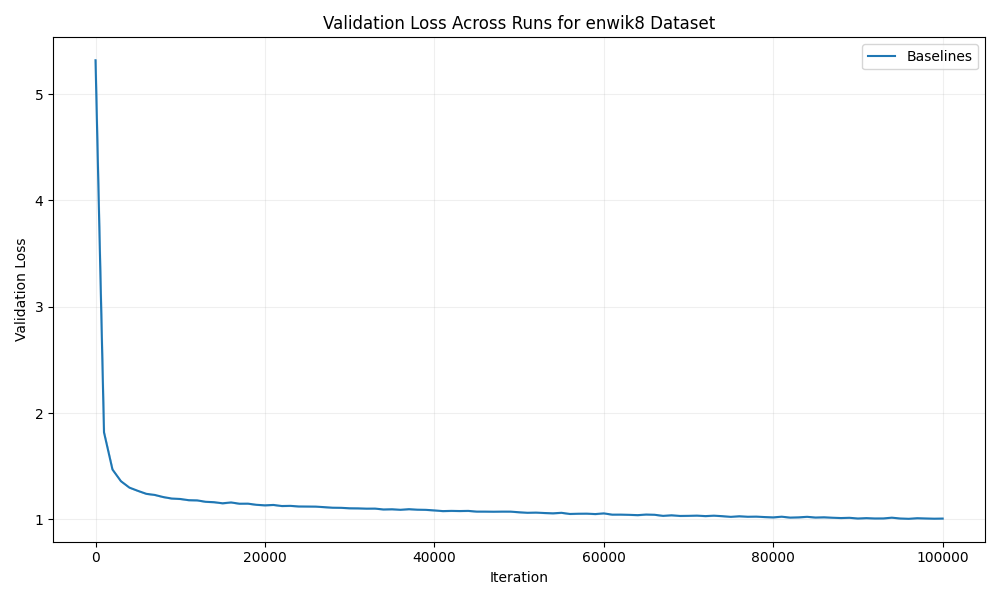
\includegraphics[width=\textwidth]{val_loss_enwik8.png}
        \caption{Validation loss.}
        \label{fig:first-run}
    \end{subfigure}
    \hfill
    \begin{subfigure}{0.49\textwidth}
        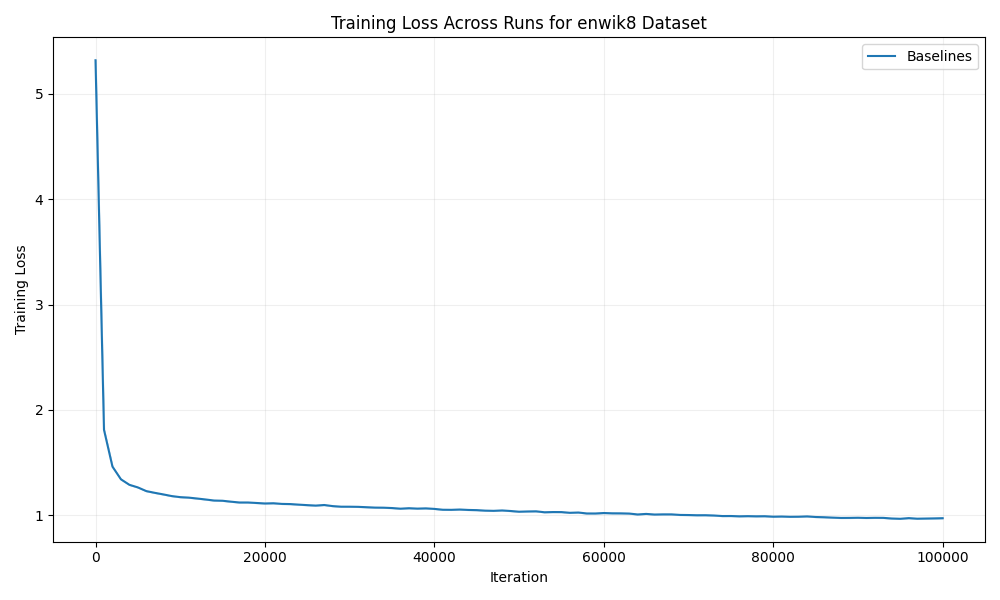
\includegraphics[width=\textwidth]{train_loss_enwik8.png}
        \caption{Training loss.}
        \label{fig:second-run}
    \end{subfigure}
    \caption{Training and validation loss for the enwik8 dataset under Adaptive Stochastic Depth. The validation loss is comparable to the baseline, while the training loss stays higher due to the regularization effect of stochastic depth.}
    \label{fig:first-figure}
\end{figure}

\section{Conclusions and Future Work}
\label{sec:conclusion}

% This paragraph summarises the motivation, method and key findings.
We introduced \textit{Adaptive Stochastic Depth}, a lightweight online controller that dynamically adjusts the block‑skip probability of Transformer models based on the validation loss EMA. By monitoring the plateau of the smoothed validation loss, our method automatically applies stronger regularization when overfitting is detected and relaxes it when the model can still benefit from increased capacity. The controller requires no additional learned parameters, adds negligible computational overhead, and can be retrofitted to any existing architecture with a single non‑persistent buffer.

% This paragraph summarises experimental results.
Experiments on three character‑level language modeling benchmarks—shakespeare\_char, enwik8, and text8—demonstrate that Adaptive Stochastic Depth substantially reduces training time while incurring minimal loss degradation. On the smallest dataset, training time drops by 17\% and the best validation loss remains virtually identical to the no‑drop baseline (1.47~vs.\ 1.47 nats). On the larger enwik8 and text8 corpora, training time is reduced by factors of \(15.9\times\) and \(15.0\times\), respectively, with validation loss increases of less than \(0.4\)~nats. The block‑skip probability trajectory evolves smoothly in response to the loss landscape, providing an interpretable signal of overfitting. These results show that a simple, loss‑driven adaptation can replace hand‑crafted stochastic depth schedules, yielding models that are both efficient and robust.

% This paragraph discusses directions for future work.
Several avenues remain open for future investigation. First, scaling the method to larger models and subword‑level tasks will test the generality of the approach across more demanding regimes. Second, while our controller uses a single threshold \(\varepsilon\) and fixed step \(\delta\), more sophisticated update rules—for example, incorporating momentum or layer‑wise probabilities—could further improve the adaptation speed. Third, the counter‑intuitive inference throughput drop observed on text8 warrants a deeper analysis of how stochastic depth interacts with autoregressive decoding. Finally, exploring the synergy with other adaptive mechanisms, such as learning‑rate schedules or adaptive dropout, may lead to fully self‑regulating training pipelines.

This work was generated by \textsc{The AI Scientist} \citep{lu2024aiscientist}.

\nocite{*}
\bibliographystyle{plain}
\bibliography{paper}

\end{document}
